\section{Relative Error and Graphic Analysis}
\label{sec:erroranalysis}


\subsection{Topic I}
\label{subsec:first_topic_error}

\begin{figure}[H]

\begin{subfigure}{0.5\textwidth}
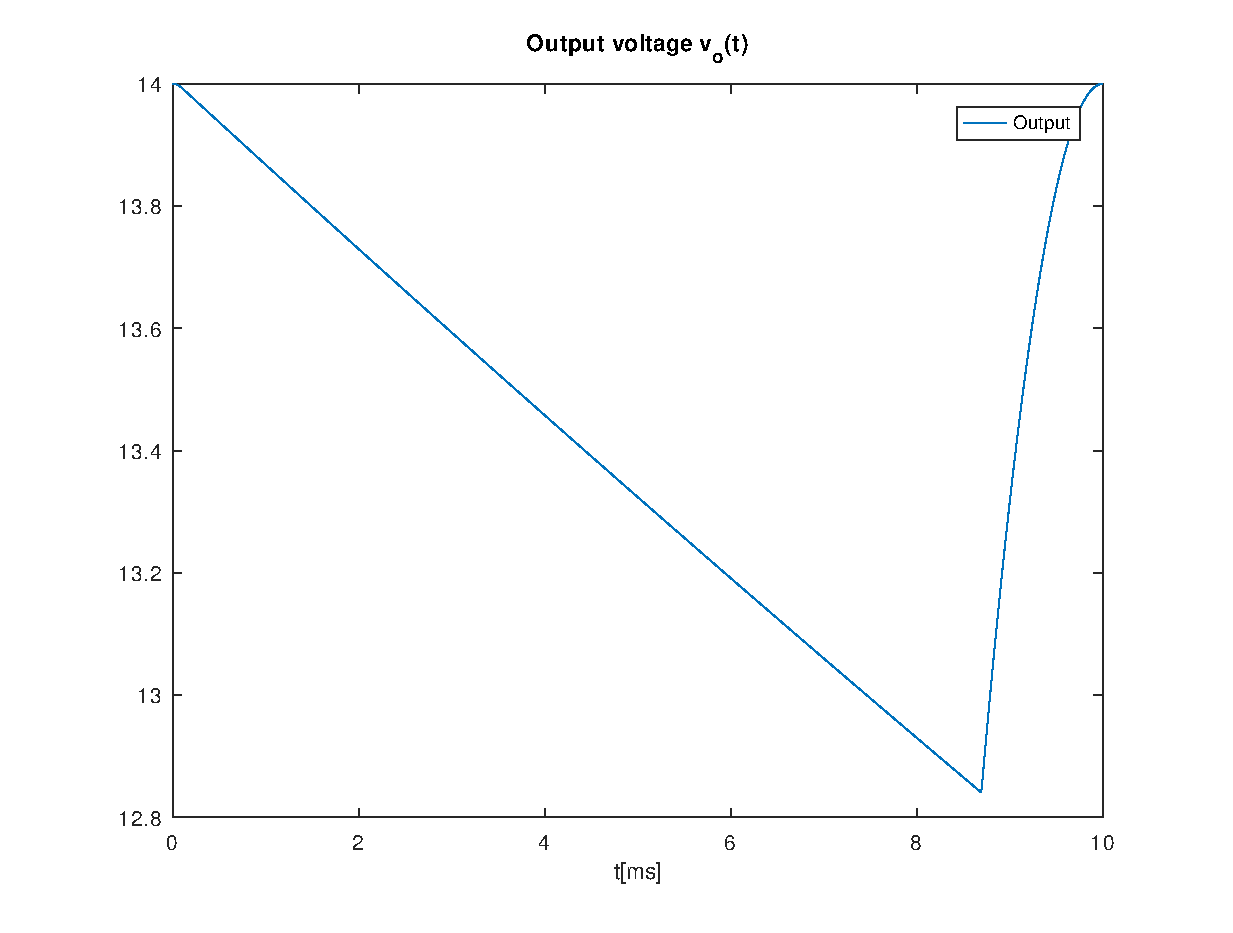
\includegraphics[width=0.9\linewidth, height=10cm]{envelope.eps} 
%\caption{}
\label{fig:theofirstcompare}
\end{subfigure}
\begin{subfigure}{0.5\textwidth}
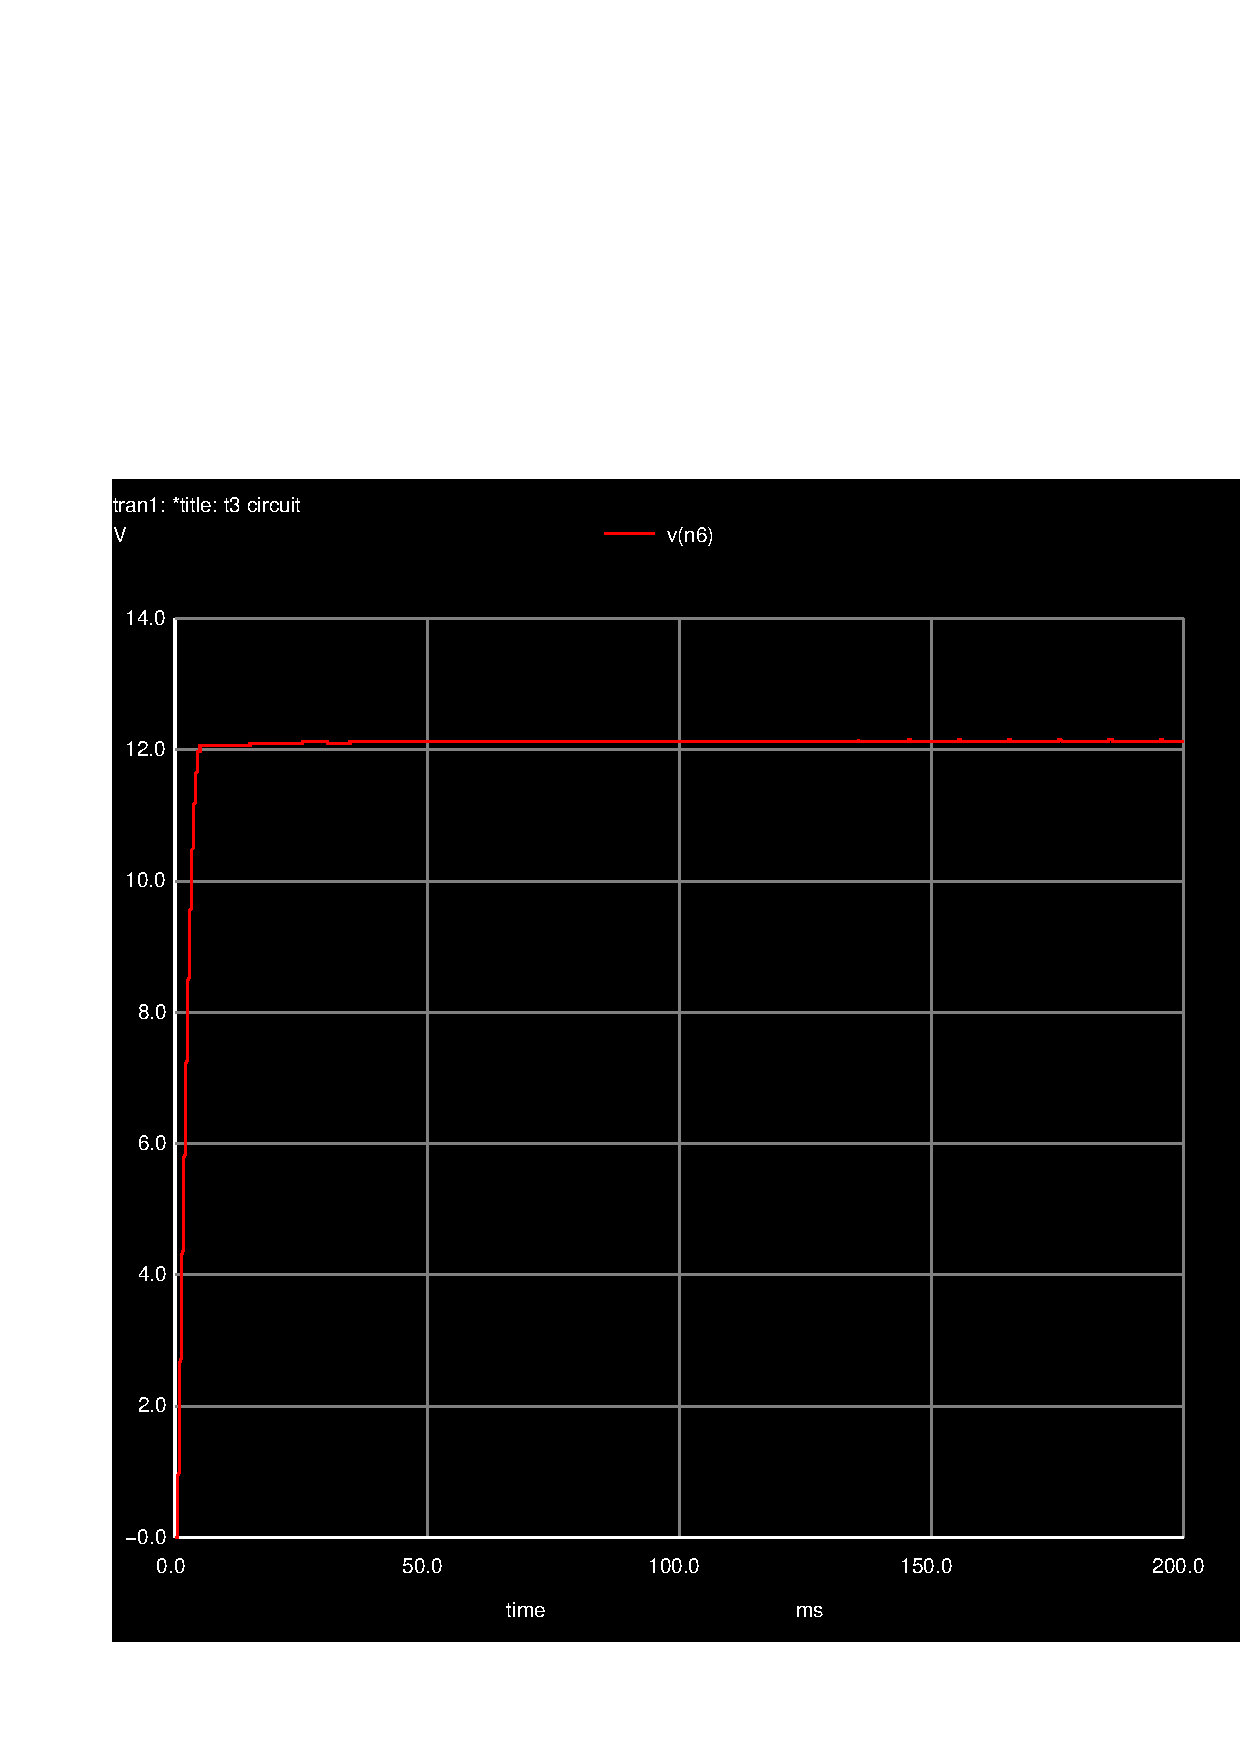
\includegraphics[width=0.9\linewidth, height=10cm]{trans1.pdf}
%\caption{}
\label{fig:simfirstcompare}
\end{subfigure}

%\caption{}
\label{fig:compar1}
\end{figure}

In first set of graphics, we have the comparation of the envelope circuits. The graphics do match our expectations in terms of results, with both already having very close numbers to $12V$


\subsection{Topic II}
\label{subsec:second_topic_error}
\begin{figure}[H]

\begin{subfigure}{0.5\textwidth}
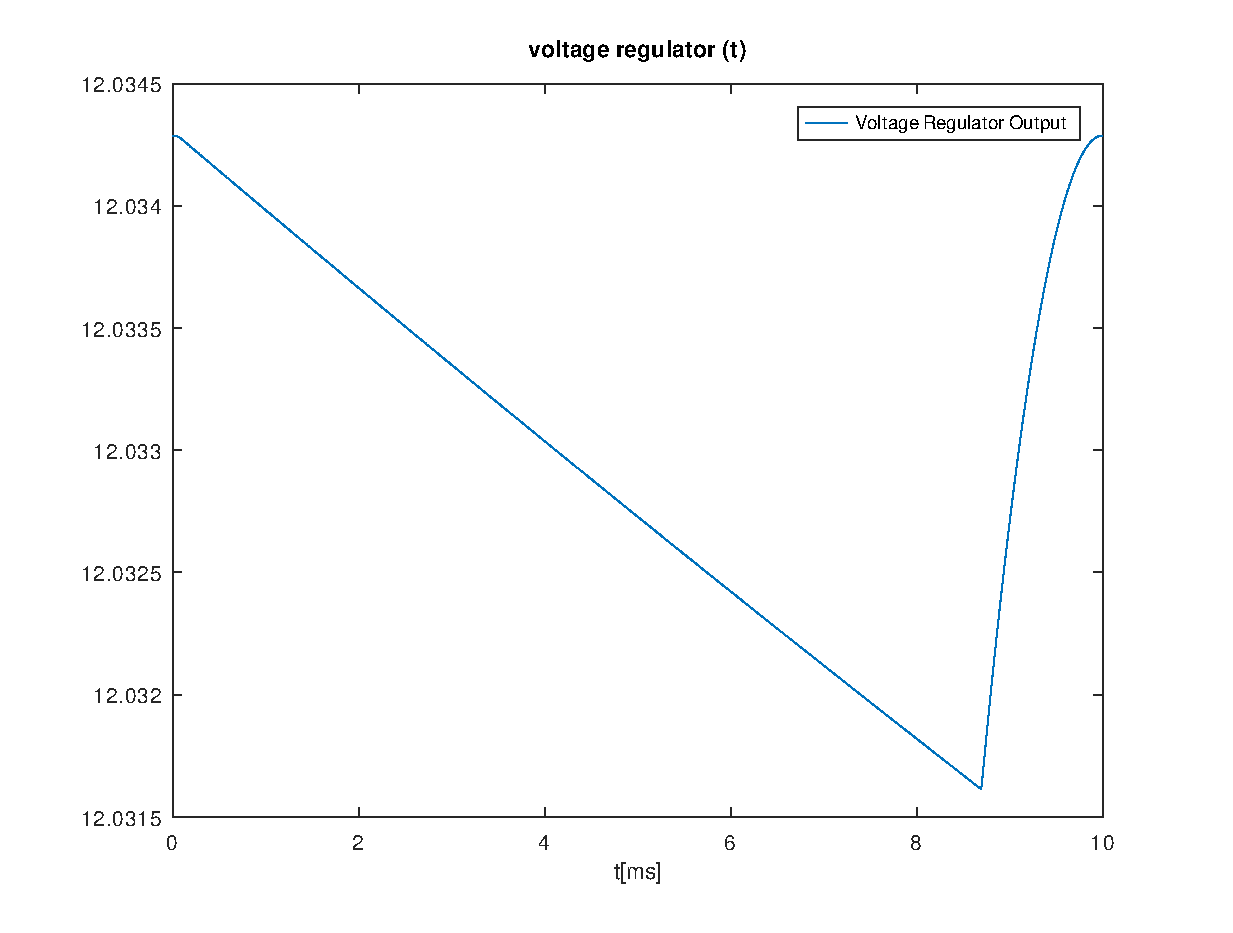
\includegraphics[width=0.9\linewidth, height=10cm]{output.eps} 
%\caption{}
\label{fig:theosecondcompare}
\end{subfigure}
\begin{subfigure}{0.5\textwidth}
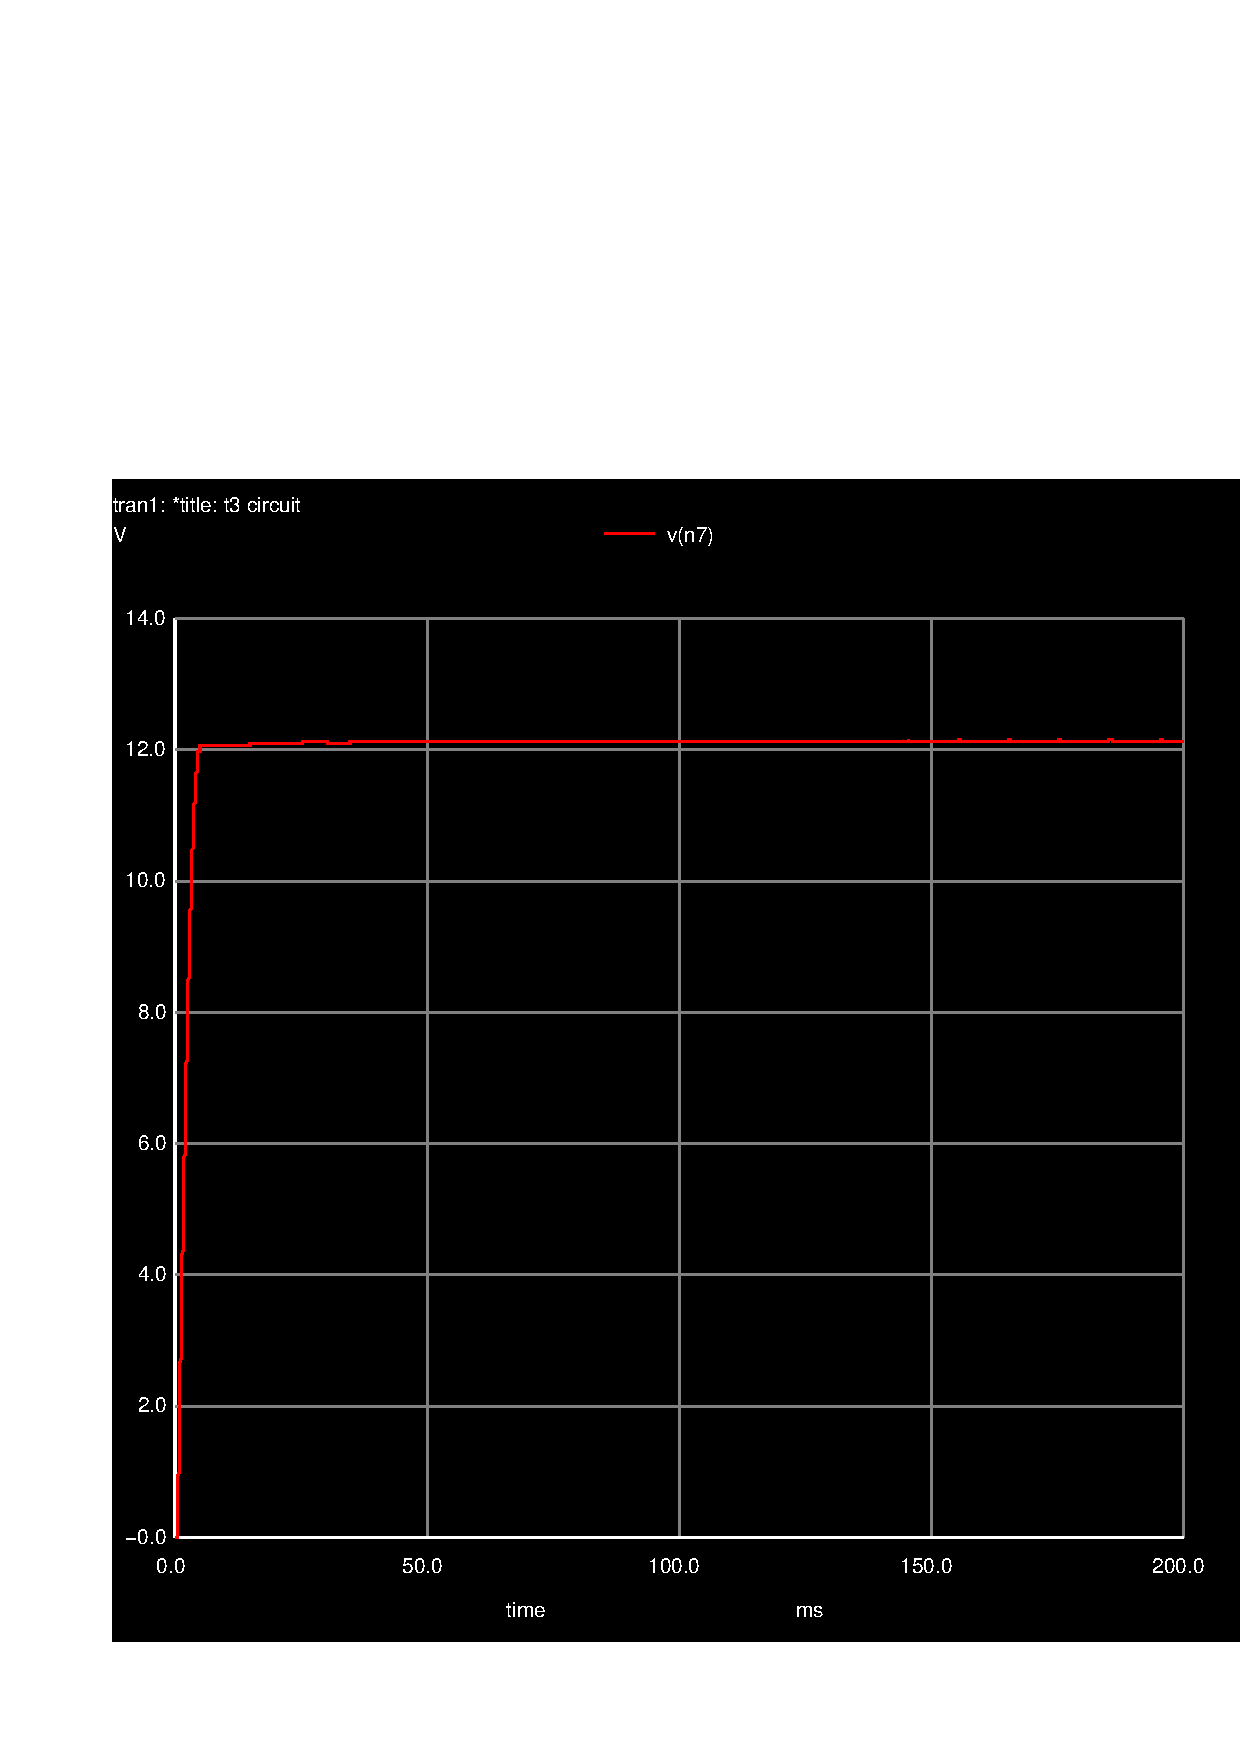
\includegraphics[width=0.9\linewidth, height=10cm]{trans2.pdf}
%\caption{}
\label{fig:simsecondcompare}
\end{subfigure}

%\caption{}
\label{fig:compar2}
\end{figure}

In this second set of graphics, we have the comparation of the output between Octave and Ngspice. Once again, the results are very sastisfying.

\subsection{Topic III}
\label{subsec:third_topic_error}


\begin{figure}[H]

\begin{subfigure}{0.5\textwidth}
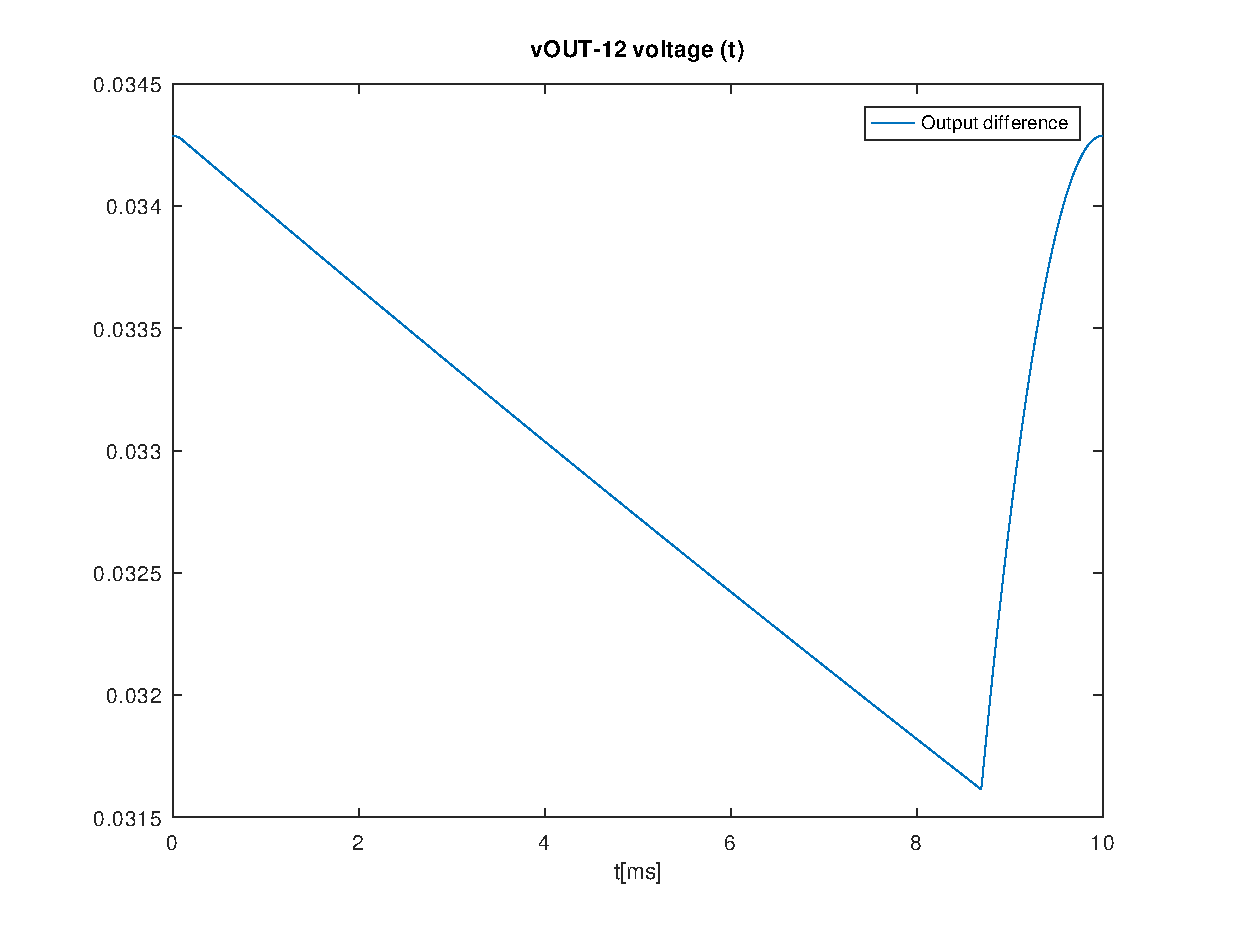
\includegraphics[width=0.9\linewidth, height=10cm]{outputdiff.eps} 
%\caption{}
\label{fig:theothirdcompare}
\end{subfigure}
\begin{subfigure}{0.5\textwidth}
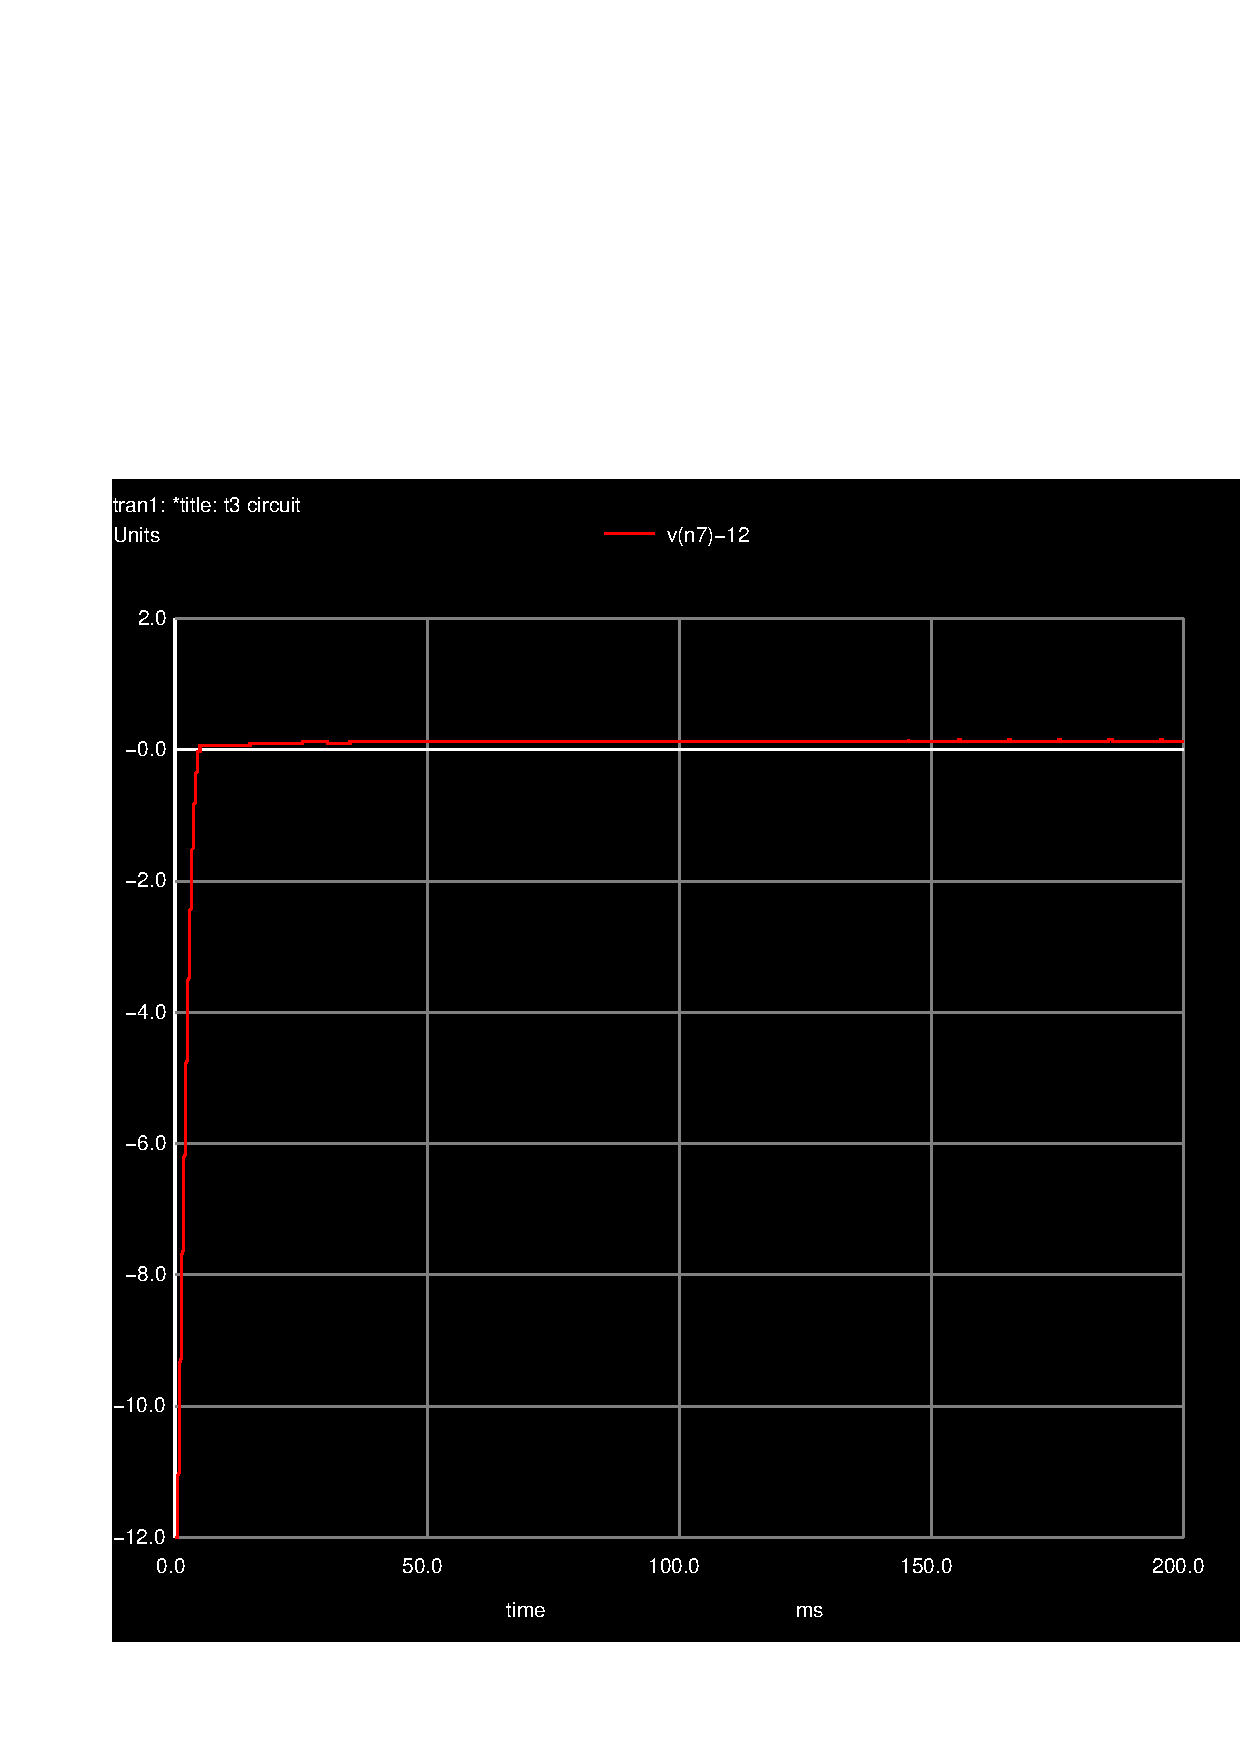
\includegraphics[width=0.9\linewidth, height=10cm]{trans3.pdf}
%\caption{}
\label{fig:simthirdcompare}
\end{subfigure}

%\caption{}
\label{fig:compar3}
\end{figure}

In this last set of graphics, we have the comparation between the output difference (relative to $12V$) obtained by Octave and Ngspice, which also correspond to what was required (as close to zero as possible).

\subsection{Topic IV}
\label{subsec:fourth_topic_error}

\begin{center}
   \begin{tabular}{|c||c|c|c|}
      \hline    
      \multicolumn{4}{|c|} {\bf Comparation of various data between Octave and Ngspice} \\
      \hline
        
 Node 1 & 5.029246e+00         & 5.02924600001e+00 & 1.98836979289e-10 \\ \hline 
 Node 2 & 4.783544e+00         & 4.78354415384e+00 & 3.21593851440e-06 \\ \hline 
 Node 3 & 4.288147e+00        & 4.28814736170e+00 & 8.43484611997e-06 \\ \hline 
 Node 4 & 4.817533e+00         & 4.81753272504e+00 & 5.70752959068e-06 \\ \hline 
 Node 5 & 5.579905e+00         & 5.57990489781e+00 & 1.83143454860e-06 \\ \hline 
 Node 6 & -1.85471e+00         & -1.85471262435e+00 & 1.41496768946e-04 \\ \hline 
 Node 7 & -2.77162e+00         & -2.77162277031e+00 & 9.99527366038e-05 \\ \hline 
   \end{tabular}
\end{center}

In the table above, we have the comparation between Octave and Ngspice of the maximum output values, the minimum output values, the voltage ripple and the average. The percentual relative error is also included to make the interpretation of these values easier.
With the exception of the Voltage Ripple, it is safe to say that all the values are very good. When it comes to the voltage ripple, while it is true that the relative error is of 5 times of difference, it is important to note that they are still very small values. The possible explanation for this discrepancy is that Ngspice uses a diode model which does not have fixed parameters (Namely $V_{D}$), making it very hard to match the Octave results.

\subsection{Topic V}
\label{subsec:Figure of Merit}

\begin{center}
   \begin{tabular}{|c||c|}
      \hline    
      \multicolumn{2}{|c|} {\bf Figure of Merit} \\
      \hline
        Merit Figure & 0.000410 
   \end{tabular}
 \end{center}

To end our report, we present the figure of merit. It is important to remind that this figure is obtained upon the devices and values used in Ngspice and not the ones used in Octave. During our work, we struggled a bit trying to understand what the ideal value would be, given that we did not have any reference however, we did our best to make it as high as possible.
